\documentclass[12pt]{article}
\usepackage[utf8]{inputenc}
\usepackage[spanish]{babel}
\usepackage{amsmath}
\usepackage{amsfonts}
\usepackage{amssymb}
\usepackage{graphicx} 
\usepackage{float} 
\usepackage{hyperref} 
\usepackage{longtable}
\usepackage{caption}
\usepackage{subcaption} 

\usepackage[margin=1in]{geometry}

\title{Análisis de Resultados: Diseño Óptimo de Red de Distribución de Agua}
\author{Javier Sola, Martín Caballero, Bastián Jiménez, Agustín Venegas \\ \small Grupo 6}
\date{\today} 

\begin{document}

\maketitle

\begin{abstract}
Este documento presenta el análisis de los resultados obtenidos del modelo matemático de optimización para el diseño de una red de tuberías de abastecimiento de agua. Se detallan los conjuntos, parámetros, variables, función objetivo y restricciones del modelo. Además, se describe el proceso de generación de instancias de diferentes tamaños y se analiza el comportamiento de la función objetivo, la factibilidad y los tiempos de resolución utilizando el software de optimización asignado.
\end{abstract}

\clearpage
\tableofcontents
\clearpage

\section{Software Asignado}
De acuerdo con la asignación por grupos (Tabla 3 del enunciado del proyecto), el Grupo 6 ha sido asignado para utilizar el software \textbf{LPSolve}.

LPSolve es un solucionador de programas lineales y enteros mixtos de código abierto. La implementación del modelo matemático se realiza mediante la generación de archivos con formato `.lp`, los cuales son interpretados y resueltos por LPSolve. Este enfoque permite la validación del modelo formulado y el análisis de los resultados obtenidos, cuyos valores son entregados en un formato csv.

\section{Análisis de Resultados}
En esta sección, se presenta el análisis de los resultados de la ejecución del modelo de optimización sobre las instancias generadas.

\subsection{Análisis de la Función Objetivo}
Se generaron y resolvieron 6 instancias (2 pequeñas, 2 medianas y 2 grandes) utilizando LPSolve. La función objetivo representa el costo total minimizado de la red, incluyendo costos de instalación y transporte. A continuación, se presenta un resumen del comportamiento de la función objetivo a medida que crece el tamaño de la instancia.

\begin{table}[H]
    \centering
    \caption{Resultados de la Función Objetivo por Tamaño de Instancia}
    \label{tab:FO_resultados}
    \begin{tabular}{|c|c|c|c|}
        \hline
        \textbf{Instancia} & \textbf{Tamaño} & \textbf{Costo Total (Función Objetivo)} \\
        \hline
        Instancia 1 & Small & 30834,0474040404 \\
        Instancia 2 & Small & 31478,3084141414 \\
        \hline
        Instancia 1 & Medium & 60047,046967676 \\
        Instancia 2 & Medium & 72467,5619979798 \\
        \hline
        Instancia 1 & Large & 284893,537482828 \\
        Instancia 2 & Large & 333093,001845455 \\
        \hline
    \end{tabular}
\end{table}

\begin{figure}[H]
    \centering
    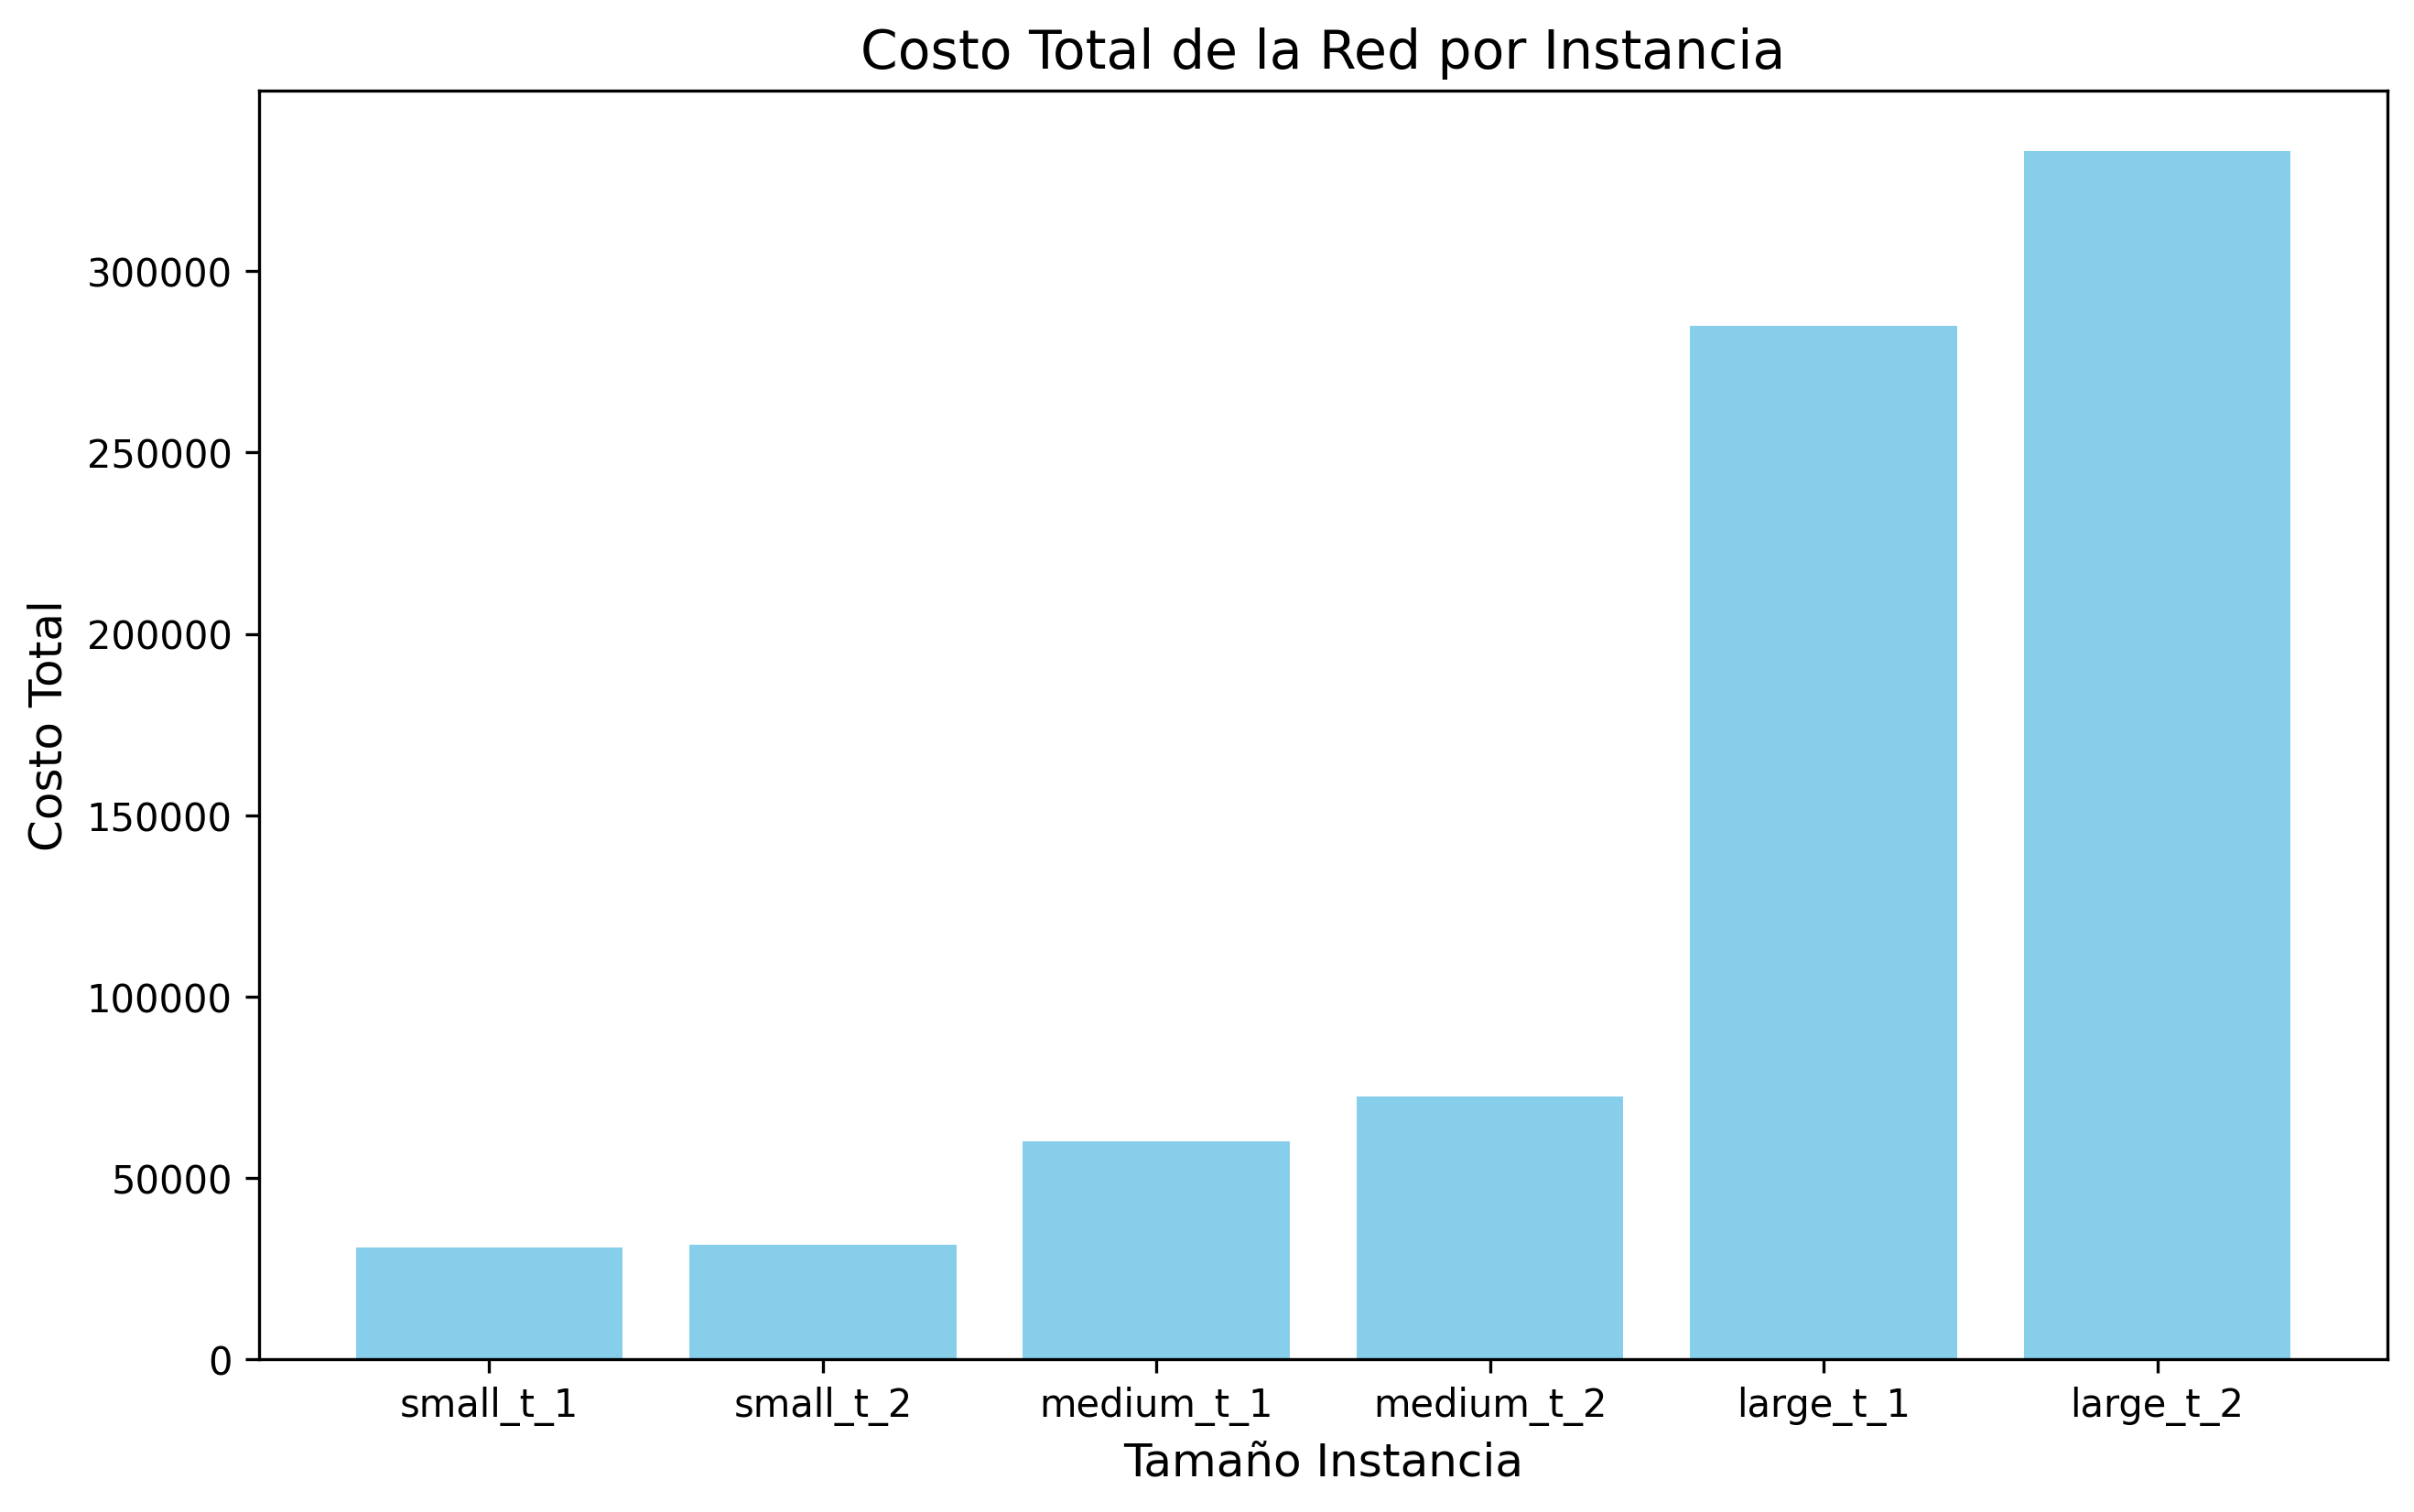
\includegraphics[width=0.8\textwidth]{of_values.png}
    \caption{Comportamiento de la Función Objetivo vs. Tamaño de la Instancia}
    \label{fig:FO_comportamiento}
\end{figure}

\textit{Discusión:}
Aqui se observa una clara tendencia al aumento del costo total de la red a medida que aumentan los valores de las instancias, sin embargo la diferencia notoria se representa más en instancias grandes, ya que en instancias pequeñas y medianas se sigue observando un orden de $10^4$, a diferencia de instancias grandes que cambian el orden de magnitud. Esta tendencia sigue la logica constituida simplemente, ya que a medida que aumenta la instancia aumentan los nodos, las tuberias, etc, simplemente se amplifica la red. Y como vemos en el grafico el tiempo tiene una tendencia exponencial.


\subsection{Análisis de Factibilidad}
La factibilidad de un problema de optimización indica si existe al menos una solución que satisfaga todas las restricciones. Es crucial para asegurar que el modelo es bien formulado y que las instancias son resolubles. Como nosotros generamos las instancias y despues el software LPsolve se encargó de la resolución y el calculo podemos dar fé de que en todas as instancias probadas nos dieron soluciones factibles, y en su consecuencia óptimas(dado que el software busca la solución óptima), lo que significa que nuestro modelo es conciso y consistente, sumado a nuestra generación de instancias.
\subsection{Dibujo}
OH CTM QEU PAJA LOKO

\section{Análisis de Tiempos de Resolución}
Se analizó el tiempo que LPSolve tarda en encontrar la solución óptima para las diferentes instancias, a medida que aumenta el tamaño del problema. Este análisis es fundamental para entender la escalabilidad del modelo.

\begin{table}[H]
    \centering
    \caption{Tiempos de Resolución por Tamaño de Instancia}
    \label{tab:Tiempos_resolucion}
    \begin{tabular}{|c|c|c|c|}
        \hline
        \textbf{Instancia} & \textbf{Tamaño} & \textbf{Tiempo de Resolución [segundos]} \\
        \hline
        Instancia 1 & Small & 0.014 \\
        Instancia 2 & Small & 0.013 \\
        \hline
        Instancia 1 & Medium & 0.072 \\
        Instancia 2 & Medium & 1.728 \\
        \hline
        Instancia 1 & Large & 3.028 \\
        Instancia 2 & Large & 4.228 \\
        \hline
    \end{tabular}
\end{table}

\begin{figure}[H]
    \centering
    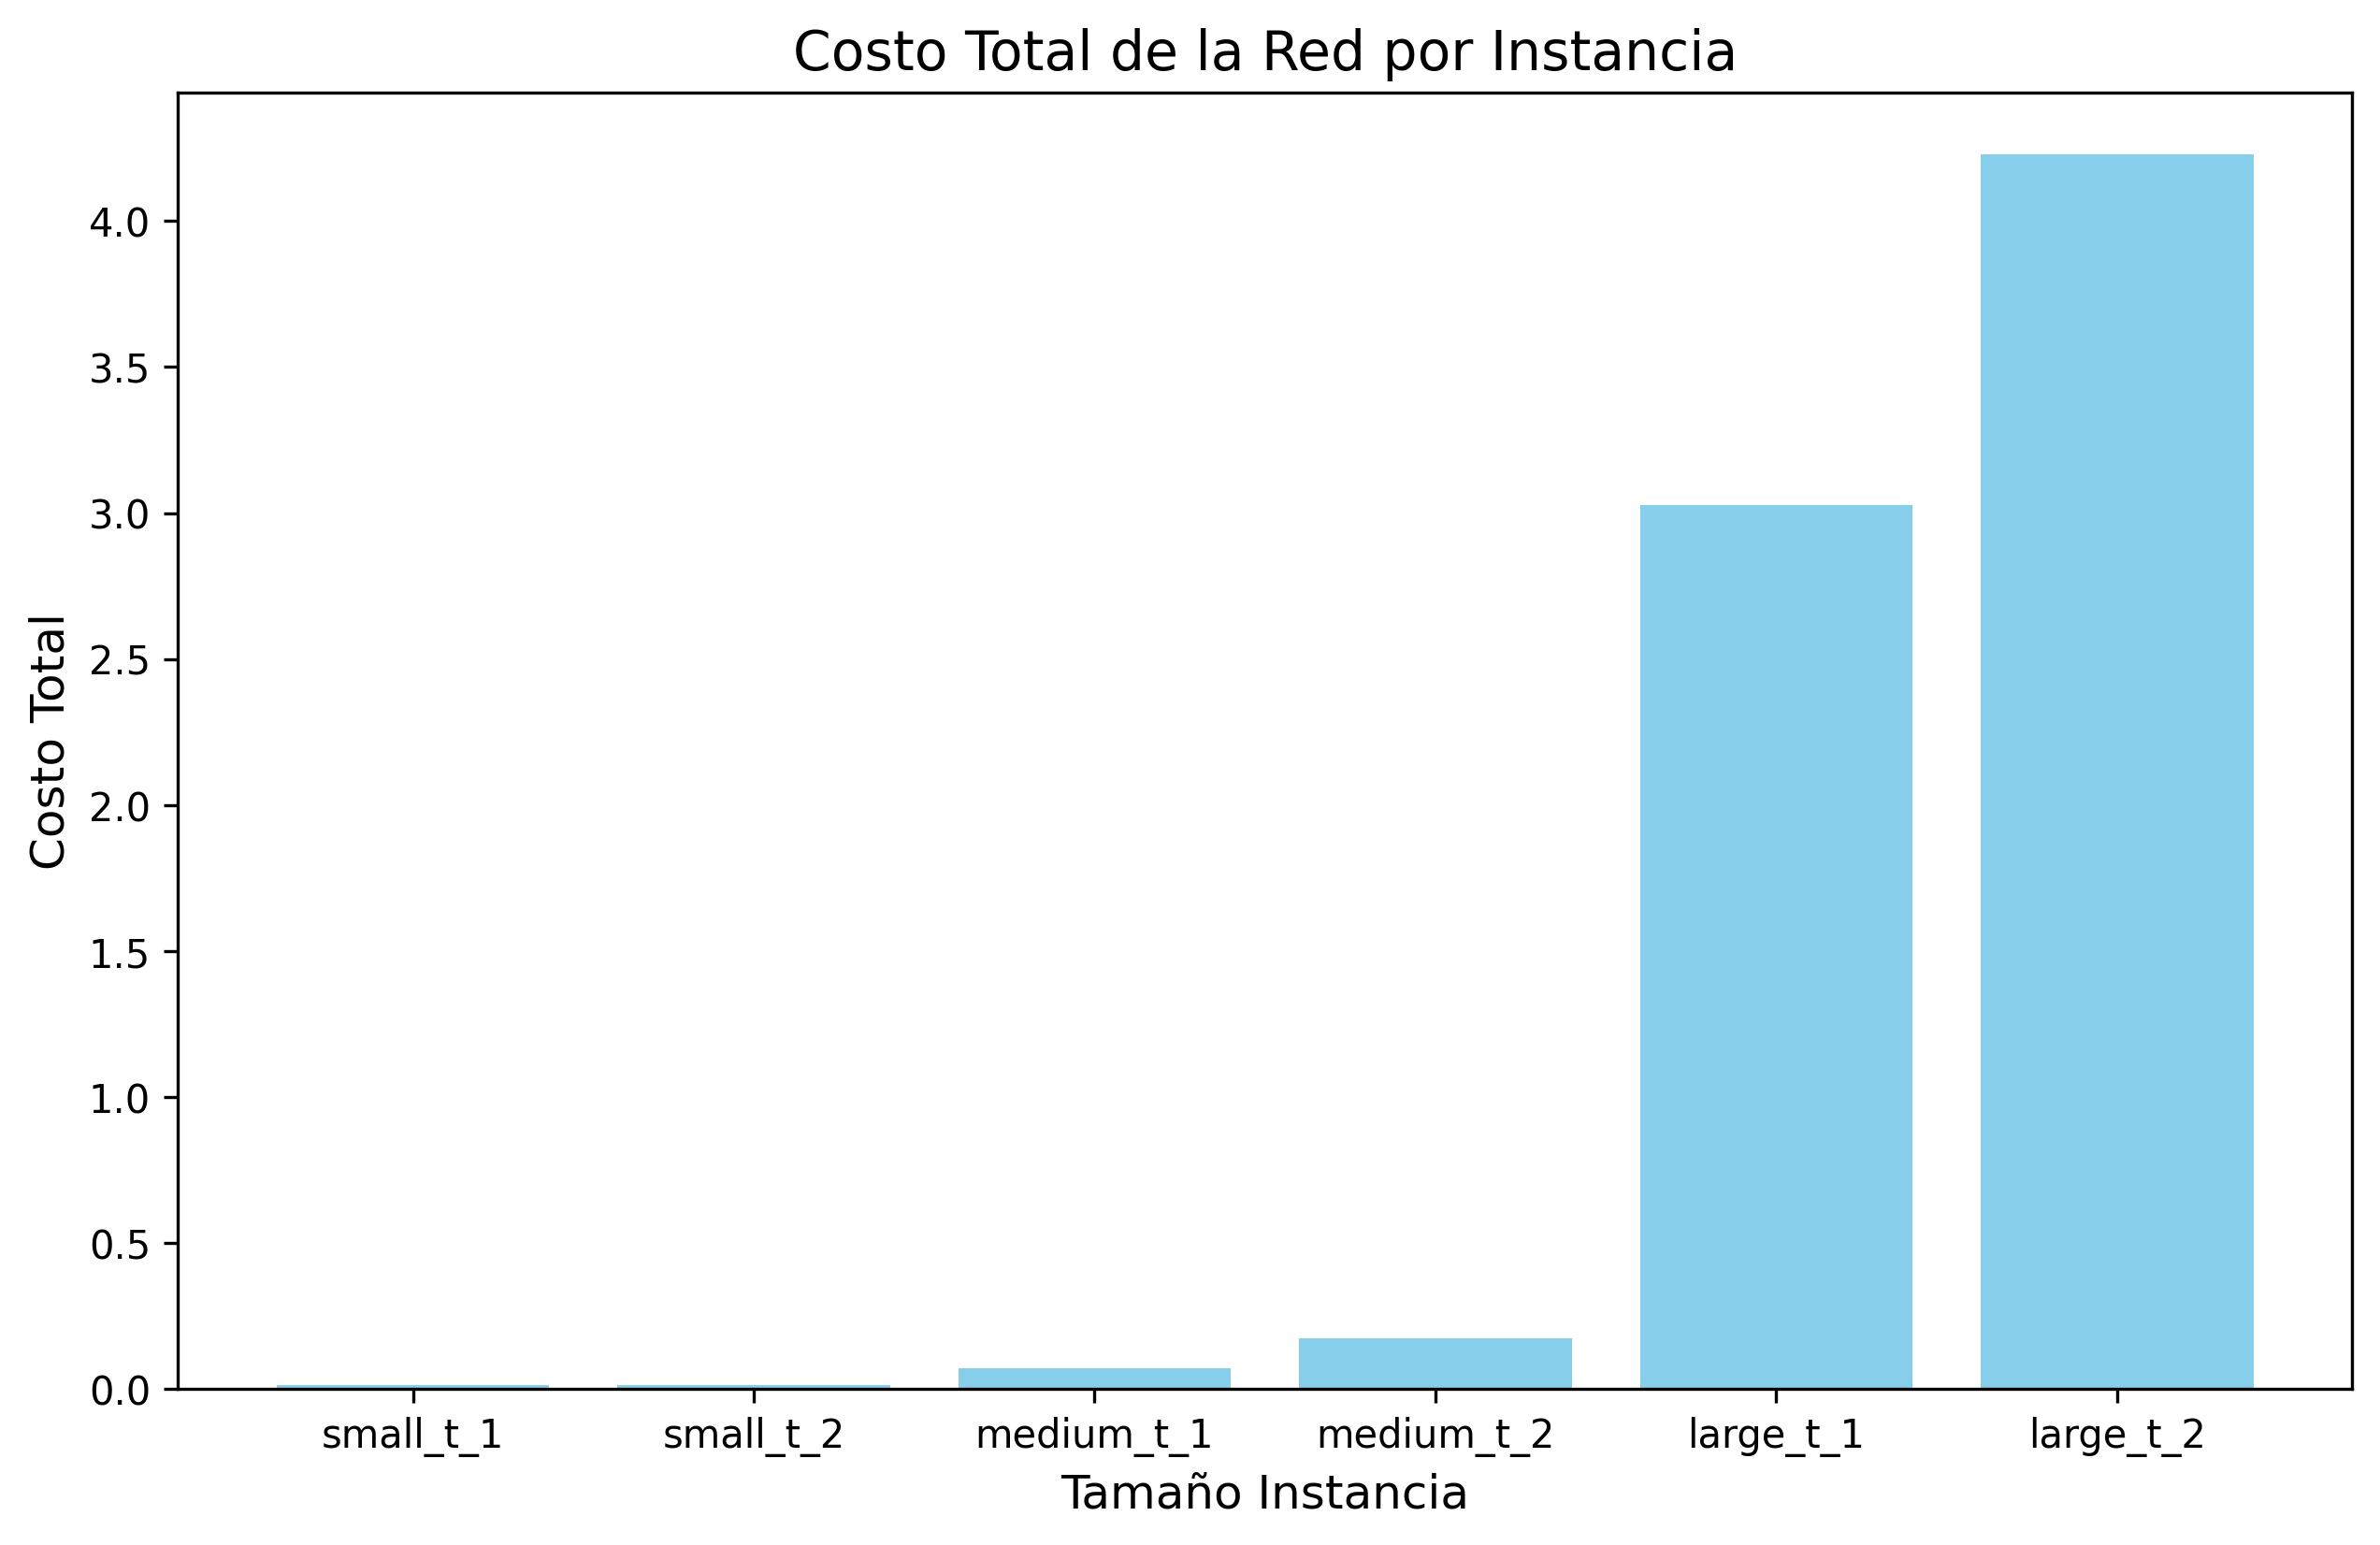
\includegraphics[width=0.8\textwidth]{time_values.png}
    \caption{Comportamiento del Tiempo de Resolución vs. Tamaño de la Instancia}
    \label{fig:tiempo_comportamiento}
\end{figure}

\textit{Discusión:}
El tiempo de resolución como vemos tiene una tendencia clara a aumentar en conjunto aumenta el tamaño de la instancia, como vemos muestras chicas se logran con diferencias de milisegundos, las medianas con milisegundos tambien pero las grandes ya se diferencian por segundos. Si vemos los graficos y analizamos que los tamaños aumentan tanto los nodos como las tuberias y etc, sabremos reconocer que son muchas variables a considerar pero la tendencia en función del tamaño de la instancia crece a ordenes muy cercanos a exponencial o exponencial, esto por la cantidad de variables a considerar que crecen linealmente y afectan la red de manera exorbitante. Un dato mas a considerar es que si comparamos los graficos de tiempo y costo a pesar de verse un poco distintos tambien siguen una misma tendencia y es que al ser la función objetivo una función monotona creciente y de manera lineal crece en conjunto al tiempo que se demora, esto multiplicado por una constante que hace que los casos menores como small se vean un poco mas grande en la tendencia, pero para instancias muy grandes los graficos de tiempo y costos se verian muy parecidos.
\end{document}